
To test GPT-3's ability to learn novel symbolic manipulations from a few examples, we designed a small battery of 5 ``character manipulation'' tasks.  Each task involves giving the model a word distorted by some combination of scrambling, addition, or deletion of characters, and asking it to recover the original word.  The 5 tasks are:

\begin{table}
    \centering
        \begin{tabular}{l l l l l l}
        \toprule
        Setting & CL & A1 & A2 & RI & RW \\ 
        \midrule
        GPT-3 Zero-shot & 3.66 & 2.28 & 8.91 & 8.26 & 0.09 \\
        GPT-3 One-shot & 21.7 & 8.62 & 25.9 & 45.4 & 0.48 \\ 
        GPT-3 Few-shot & 37.9 & 15.1 & 39.7 & 67.2 & 0.44 \\ 
        \bottomrule
        \end{tabular}
    \caption{GPT-3 175B performance on various word unscrambling and word
manipulation tasks, in zero-, one-, and few-shot settings. CL is ``cycle letters in word'', A1 is anagrams of but the first and last letters,
A2 is anagrams of all but the first and last two letters, RI is ``Random insertion
in word'', RW is ``reversed words''.}
    \label{table:unscramble}
\end{table}
\begin{figure}
\centering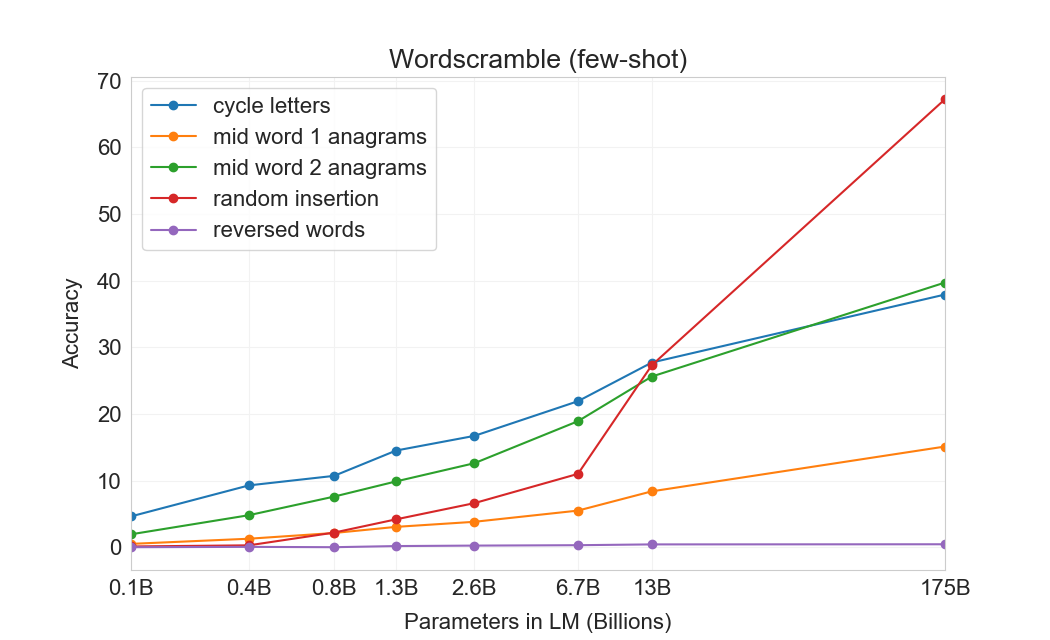
\includegraphics[width=0.8\linewidth]{graphs/scale_plots/wordscramble_fewshot.png}
\caption{Few-shot performance on the five word scrambling tasks for different sizes of model.  There is generally smooth improvement with model size although the random insertion task shows an upward slope of improvement with the 175B model solving the task the majority of the time.  Scaling of one-shot and zero-shot performance is shown in the appendix.  All tasks are done with $K=100$.}
\label{graph:scramble}
\end{figure}

\begin{itemize}
    \item \textbf{Cycle letters in word (CL)} -- The model is given a word with its letters cycled, then the ``='' symbol, and is expected to generate the original word.  For example, it might be given ``lyinevitab'' and should output ``inevitably''.
    \item \textbf{Anagrams of all but first and last characters (A1)} -- The model is given a word where every letter except the first and last have been scrambled randomly, and must output the original word.  Example: criroptuon = corruption.
    \item \textbf{Anagrams of all but first and last 2 characters (A2)} -- The model is given a word where every letter except the first 2 and last 2 have been scrambled randomly, and must recover the original word.  Example: opoepnnt $\to$ opponent.
    \item \textbf{Random insertion in word (RI)} -- A random punctuation or space character is inserted between each letter of a word, and the model must output the original word.  Example: s.u!c/c!e.s s i/o/n = succession.
    \item \textbf{Reversed words (RW)} -- The model is given a word spelled backwards, and must output the original word.  Example: stcejbo $\to$ objects.
\end{itemize}

For each task we generate 10,000 examples, which we chose to be the top 10,000 most frequent words as measured by \cite{norvig2009ngram} of length more than 4 characters and less than 15 characters. The few-shot results are shown in Figure \ref{graph:scramble}.  Task performance tends to grow smoothly with model size, with the full GPT-3 model achieving 66.9\% on removing random insertions, 38.6\% on cycling letters, 40.2\% on the easier anagram task, and 15.1\% on the more difficult anagram task (where only the first and last letters are held fixed).  None of the models can reverse the letters in a word. 

In the one-shot setting, performance is significantly weaker (dropping by half or more), and in the zero-shot setting the model can rarely perform any of the tasks (Table \ref{table:unscramble}).  This suggests that the model really does appear to learn these tasks at test time, as the model cannot perform them zero-shot and their artificial nature makes them unlikely to appear in the pre-training data (although we cannot confirm this with certainty).

We can further quantify performance by plotting ``in-context learning curves'', which show task performance as a function of the number of in-context examples.  We show in-context learning curves for the Symbol Insertion task in Figure \ref{graph:scramble_prompted}.  We can see that larger models are able to make increasingly effective use of in-context information, including both task examples and natural language task descriptions.

Finally, it is worth adding that solving these tasks requires character-level manipulations, whereas our BPE encoding operates on significant fractions of a word (on average $\sim0.7$ words per token), so from the LM’s perspective succeeding at these tasks involves not just manipulating BPE tokens but understanding and pulling apart their substructure. Also, CL, A1, and A2 are not bijective (that is, the unscrambled word is not a deterministic function of the scrambled word), requiring the model to perform some search to find the correct unscrambling. Thus, the skills involved appear to require non-trivial pattern-matching and computation.
